\chapter{Assignment and Requirements}

\section{Assignment Summary}
The whole original assignment can be found in Appendix B. In this section we just provide a short summary of the assignment. 

Massive open online courses (MOOCs) around the world are growing in size and thus the practical assignments need to be easy to manage.
The growth also means that it is more difficult for each participant to find a possible practical partner due to the large amount of people.
It also becomes really difficult to find the correct partner or group members when you don't see each other during courses and haven't even met most of the people from your course.

Most of the time participants of MOOCs are searching group members on social media like Facebook or Twitter.
They just try to look through some of the participants names in the course, search for them on-line through social media and check if they are a capable partner or group member.
This approach takes a lot of time and most of the time there are too much MOOC participants to go trough all of them.

Next to the fact that this process is very time consuming, this process also often leads to a sub optimal solution.
This is due to the problem that people often look for partners of group members which share the same interests.
While this often makes it easy to work together, this will not guarantee that you have a good functioning group and enough knowledge inside the group.

We would like to improve upon this process by creating an application that can be used to create practical groups without the participants being required to go search intensively trough all the participants.
Participants should be able to easily access the application, fill in some relevant information about themselves and then be recommended possible practical partners or group members.

The interaction with the system has some difficulties.
If we want to get some information from third parties, we are required to use the information in a way this third party delivers the data.
There can be difficulties processing this data.

The recommendation of possible group members can be quite difficult too.
One of the problems we are facing is the question: What user information is useful to determine whether two people can be good practical partners?

\section{Client and academic supervision}
During the project, we had both a TU Delft coach and a company contact.
During weekly meetings, we discussed our progress and the preferences form the client.
In Table~\ref{supervision} you can see the roles of our supervisors.

\begin{table}[H]
\begin{tabular}{ | p{3cm} | p{5cm} | p{6cm} | }
 \hline
Leon Rothkrantz & Group Mentor and Supervisor & Supervises the project from the academic point of view and aides the group with difficulties.\\ \hline
Dragos Datcu &  Client, Group Mentor and Supervisor & Supervises the project from a client point of view and aides the group with difficulties.\\
\hline
\end{tabular}
\caption{Our supervisors}
\label{supervision}
\end{table}

\section{Actors of the System}
The system can be used by three different actors.
Each of these actors can perform different actions and therefore have different requirements.
By defining the requirements, as we do in the next section, we take these different actors in account.

\subsubsection{Actor 1: MOOC participant}
Due to the nature of the MOOCs, there are no requirements set for the participants.
Every person with an interest in the given course can enlist for the MOOC and should thus be able to register with our system.
\subsubsection{Actor 2: MOOC teacher/MOOC administrator} 
The MOOC is organised by a professor of an university.
This professor will need to register with the system and create a MOOC.
\subsubsection{Actor 3: Groups of participants}
This actor consist of two or more MOOC participants who accepted each other to their group.
These groups can be of variable size, set by the MOOC organiser.

\section{Global Goals and Requirements}
To determine the direction the project should be following, we define goals for the project.
These goals will later be used to determine whether the final product is in line with these goals.
\begin{itemize}
\item The final product, that will be presented, will be a working proof of concept which will fit closely with the specified target audience and demands of the assignment.
\item We want to create a platform for searching other students, letting the students invite other students for a practical group and letting the students join each other.
\item We want the final product to recommend good fitting, possible group members to the students.
By "good fitting" we mean that there is some heuristic that we use to calculate whether two students would make a good combination.
\item We want the final product to achieve more optimal groups than the current situation by recommending other students.
\end{itemize}

The goals do not include a goal for the teachers part, because the current goals focus on the student.
This is because of the limited time of the project and the current goals having enough depth for an extensive system.
Next to this, the assignment specifically focusses on the need of the students to have a platform to search, interact with other students to form practical groups and have help with searching for their best practical group.
Although it would be beneficial for the teacher to have an easy to use platform for managing his practical assignments, it is out of the scope of this project.

To provide an overview of what actions the software must be capable of, we define four global requirements for the system.
By defining these three global requirements we provide a foundation for the detailed requirements.
\begin{itemize}
\item MOOC teachers must be able to create, manage and edit courses.
Participants of their MOOC are able to register to this course.

\item MOOC students must be able to register and deregister for a course.

\item The system must be capable to use personal data provided by the user to find a suggestion of an appropriate practical partner or group member.
It must be possible to adjust the definition (parameters) of the appropriate practical partner or group member, and search trough several suggestions.
\end{itemize}

\section{Detailed Requirements}
This section will mention the different requirements that involve the basic system which the actors interact with.
The section starts with mentioning the possible types of user information the application can use and what requirements are associated with that.
Followed up by what actions are possible within the system.
After that, the kind of system is limited by the requirements listed.
Lastly we will list the requirements set for the algorithm.

We use the MoSCoW model to divide the requirements in their appropriate categories.
The M stands for must have, the S for should have, the C for could have and the W for would have.

\subsection{User Information}
\begin{tabular}{ | p{0.5cm} | p{12cm} | p{2cm} | }
\hline
\textbf{\#} & \textbf{Requirement} & \textbf{MoSCoW} \\ \hline
1 & Users must have a viewable profile that can be filled with personal information. & M \\ \hline
2 & Users must be able to enter the following registration information during registration: Full name, Email address, Password. & M \\
3 & Users must fill in their academic performances. Which knowledge, skills and completed courses does the user have? & M \\ \hline
4 & Users should be able to enter the basic user information, like: country, age, short description, skills, education, a picture and personality traits. & S \\ \hline
5 & Users could be able to use a personality test to determine their personality traits. & C \\ \hline
6 & Users could be able to fill in their personality traits. & C \\ \hline
7 & Users could be able to enter the following extended user information: preferred group role, role of the other group members, etcetera. & C \\ \hline
8 & Users could be able to enter a predefined questionnaires. & C \\
\hline
\end{tabular}

\subsection{Usage of the System}
\begin{tabular}{ | p{0.5cm} | p{12cm} | p{2cm} | }
\hline
\textbf{\#} & \textbf{Requirement} & \textbf{MoSCoW} \\ \hline
\multicolumn{3}{|p{14.5cm}|}{\textbf{Actor 1: MOOC participant}} \\ \hline
1 & The potential participant (anyone who visits the site) must be able to view the different MOOCs without registering or logging in. & M \\ \hline
2 & The participant must be able to inform him/herself about the usage of the application without registering or logging in. & M \\ \hline
3 & The participant must be able to register to the application. & M \\ \hline
4 & The participant must be able to log in to the application. & M \\ \hline
5 & The participant must be able to register to the MOOCs which they were enlisted for (known to the administrator). & M \\ \hline
6 & The participant must be able to view a possible practical partner. & M \\ \hline
7 & The participant must be able to communicate with the possible practical partner to verify the matching. & M \\ \hline
8 & The participant must be able to accept or decline the practical partner into his practical group. & M \\ \hline
9 & The participant must be able to communicate within the group. & M \\ \hline
10 & The participant should be able to ask a currently existing group if he can join them. & S \\ \hline
11 & The participant should be able to use their LinkedIn profile to log in to the application. & S \\ \hline
12 & In case the participant already has an account, the participant should be able to add the course to his profile using the teachers url. & S \\ \hline
13 & The participant should be able to receive an invitation from a group. & S \\ \hline
14 & The participant should be able to accept the invitation from a group. & S \\ \hline
15 & The participant could be able to set his preferences for his possible partner. & C \\ \hline
16 & The participant could be able to search for other participants using information that is available in the profile. & C \\ \hline
\end{tabular}
\begin{tabular}{ | p{0.5cm} | p{12cm} | p{2cm} | }
\hline
\multicolumn{3}{|p{14.5cm}|}{\textbf{Actor 2: MOOC teacher/MOOC administrator}} \\ \hline
17 & The administrator must be able to create a course and add this to his account. & M \\ \hline
18 & The administrator must be able to create an url that he can use to invite the participants. & M \\ \hline
19 & The administrator must be able to manage the list of participants and groups of participants. & S \\ \hline
20 & The administrator must be able to open and close the participant registration for a course. & S \\ \hline
21 & The administrator should be able to set a deadline for a practical. & S \\ \hline
22 & The administrator should be able to communicate with every participant. & S \\ \hline
23 & The administrator should be able to communicate with the groups. & S \\ \hline
24 & The administrator should be able to grade the group for its practical. & C \\ \hline
25 & The administrator could be able to provide for his own criteria for each of his course. & C \\ \hline
26 & The administrator could be able to add different assignments to the application. & C \\ \hline
27 & The administrator could be able to view what groups have finished what assignments. & C \\ \hline
28 & The administrator could be able to grade the different assignments. & C \\ \hline
29 & The administrator could be able to provide feedback for the different assignments. & C \\ \hline
\end{tabular}
\begin{tabular}{ | p{0.5cm} | p{12cm} | p{2cm} | }
\hline
\multicolumn{3}{|p{14.5cm}|}{\textbf{Actor 3: Groups of participants}} \\ \hline
30 & A group should be able to view a possible group member. & S \\ \hline
31 & A group should be able to invite a possible group member to join their group. & S \\ \hline
32 & A group should be able to accept an request from a participant to join their group. & S \\ \hline
33 & The groups must be able to communicate with each other using the application. & C \\ \hline
34 & The group could be able to select their preferences for the new group member. & C \\ \hline
35 & The participants could be able to share files to other group members using this application. & C \\ \hline
36 & The participants would be able upload their source code to the application for verification. & W \\
\hline
\end{tabular}

\subsection{Kind of System}
\begin{tabular}{ | p{0.5cm} | p{12cm} | p{2cm} | }
\hline
\textbf{\#} & \textbf{Requirement} & \textbf{MoSCoW} \\ \hline
1 & The application must be easily accessible to both participants and course organizers. & M \\ \hline
2 & The system must provide account management functionality. & M \\ \hline
3 & The system must use a database to store the different data put in by the user. & M \\ \hline
4 & The system could be able to be combined with practical systems already used by MOOC organizers. & C \\
\hline
\end{tabular}

\subsection{Peer Matching}
\begin{tabular}{ | p{0.5cm} | p{12cm} | p{2cm} | }
\hline
\textbf{\#} & \textbf{Requirement} & \textbf{MoSCoW} \\ \hline
1 & The algorithm must be able to use a list of users as input. & M \\ \hline
2 & The algorithm must deal with continuous variation in amount of users. & M \\ \hline
3 & The algorithm must be able to return one or more suggestions of practical partners to the user given a list of rejected users. & M \\ \hline
4 & The algorithm must be able to return one or more suggestions of possible groups the participant could join. & M \\ \hline
5 & The algorithm uses basic user provided data (e.g. education, preferences) to build up a profile for a course participant. & S \\ \hline
6 & The algorithm can calculate whether two people will be good practical partners using the basic user provided data. & S \\ \hline
7 & The algorithm can return a possible practical partners using the basic user provided data. & S \\ \hline
8 & The algorithm uses advanced user provided data (e.g. asked questions, programming tests) to build up an extended profile for a course participant. & C \\ \hline
9 & The algorithm can calculate whether two people will be good practical partners using the advanced user provided data. & C \\ \hline
10 & The algorithm can return a possible practical partner using the basic user provided data. & C \\ \hline
11 & The algorithm could be able to respond to the preferences of groups. & C \\ \hline
12 & The algorithm could be able to respond to the preferences of a participant. & C \\ \hline
13 & The algorithm would have to be able to use information gathered from rejections to improve the matching. & W \\
\hline
\end{tabular}

\section{Changed requirements}
During the project we noticed that some requirements were not classified properly.
These requirements do not have the priority that we initially thought they would have.
Following the goals that we have set for the final product, we reasoned that these requirements were not must haves for the final product.
The teacher part of the system is something we would want to look into, the moment that the final product has a focus towards actual use and not at the proof of concept phase.
Below we listed the requirements that were reclassified.
We have listed both the old and new classification.
\begin{tabular}{ | p{0.5cm} | p{10cm} | p{2cm} | p{2cm} | }
\hline
\textbf{\#} & \textbf{Requirement} & \textbf{Old MoSCoW classification} & \textbf{New MoSCoW classification} \\ \hline
19 & The administrator must be able to manage the list of participants and groups of participants. & M & S \\ \hline
20 & The administrator must be able to open and close the participant registration for a course. & M & S \\ \hline
33 & The groups must be able to communicate with each other using the application. & M & C \\ \hline
\end{tabular}



\section{Graphical User Interface Mockups}
We have multiple important features in our application.
Each of these features has an own graphical user interface (GUI).
Below, we will provide mockups from the graphical user interfaces of the most important features.

\subsection{Profile}
As you can see in Figure~\ref{mockup_profile}, you can view someone's (or your own) profile.
You can see the basic profile information which the user has filled in himself.

If you are looking for a practical partner, you can get a better impression of that person when you get an overview of the profile information of that person.
This is just a simple page, because you should quickly get an impression of the student.\\

\begin{figure}[H]
    \centering
    \captionsetup{justification=centering}
    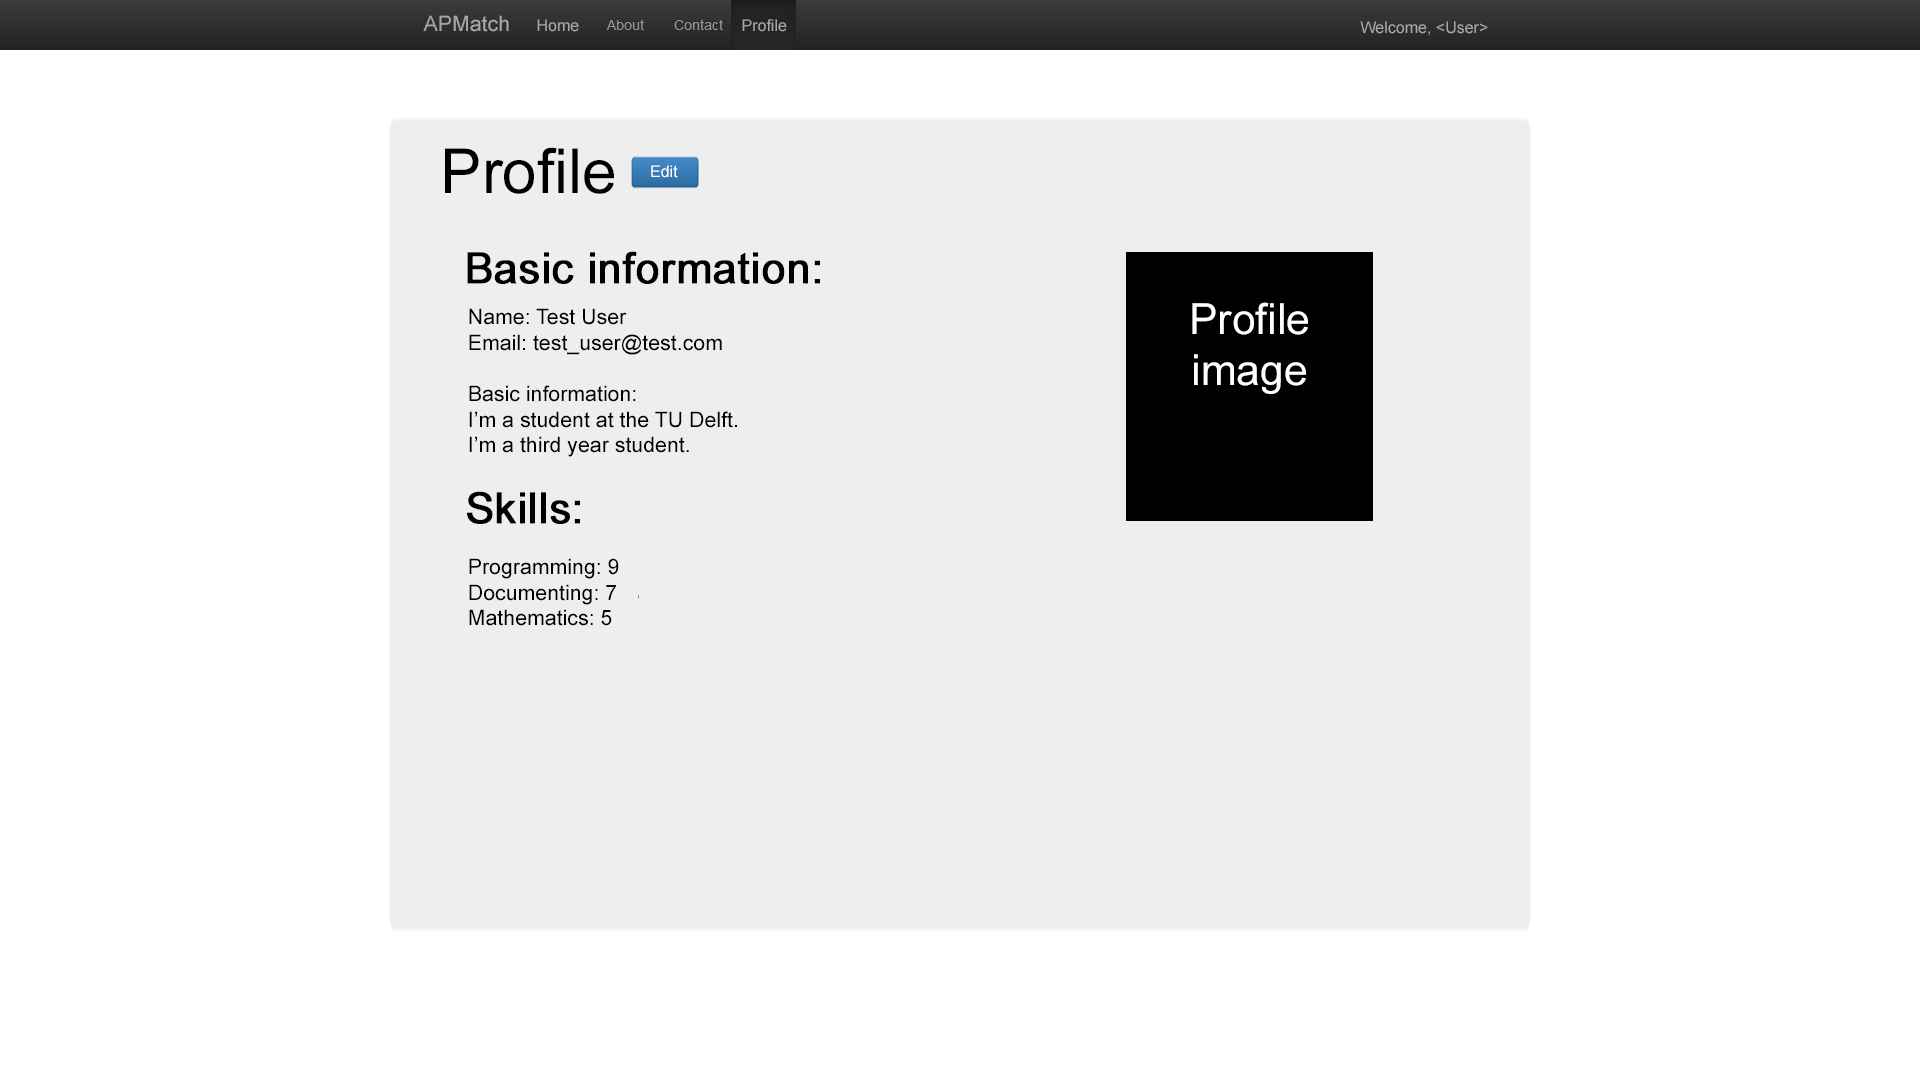
\includegraphics[width=\textwidth, frame]{images/mockup_profile}
    \caption{Interface for the profile page}
    \label{mockup_profile}
\end{figure}

In Figure~\ref{mockup_edit_profile}, you see the page for editing your profile.
On this page, you can edit your basic profile information as well as the level of your skills.
You can also change your password and your profile image.
This information will be taken into account while determining the recommended practical partners.
So it is important for the users to be able to fill in this information easily.

\begin{figure}[H]
    \centering
    \captionsetup{justification=centering}
    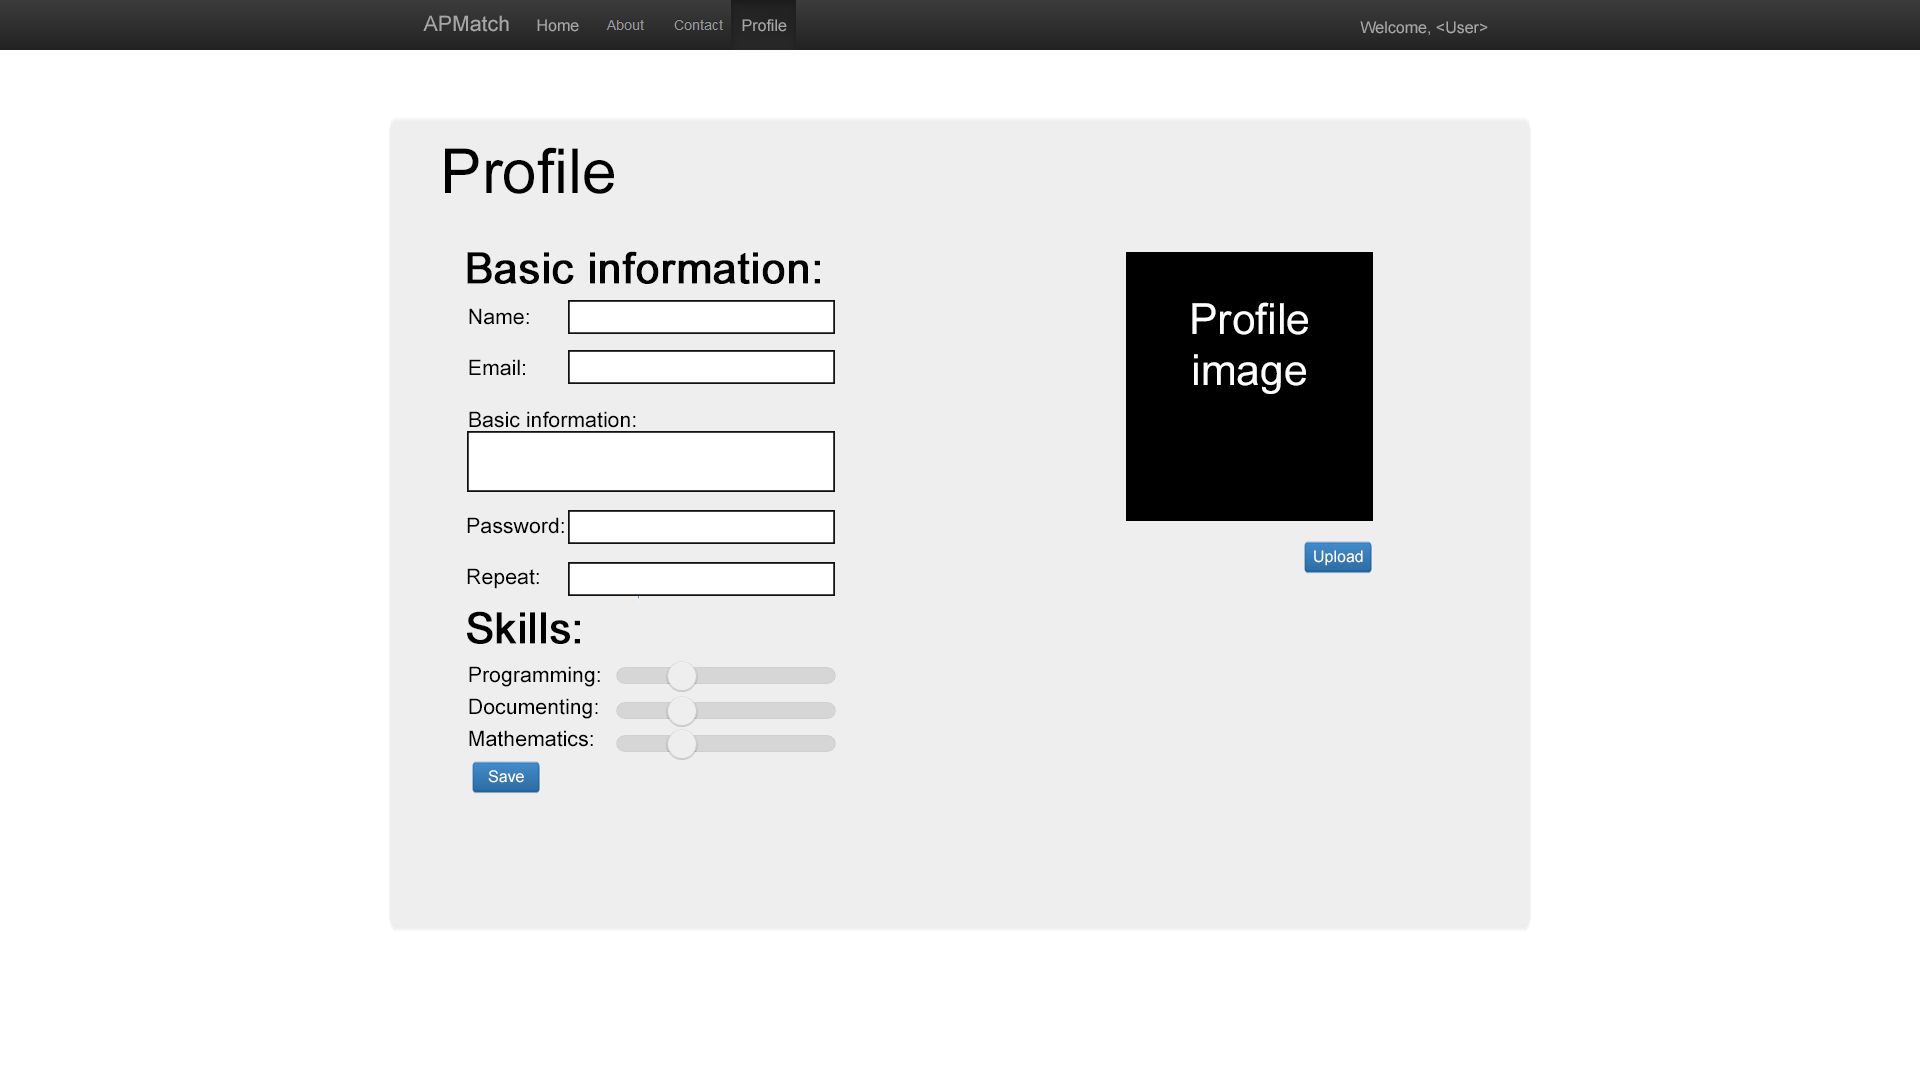
\includegraphics[width=\textwidth, frame]{images/mockup_edit_profile}
    \caption{Interface for editing the profile}
    \label{mockup_edit_profile}
\end{figure}

\subsection{Practical}
The main feature in our application is recommend practical partners.
Therefore, the users need to be able to register for a practical assignment.
The users receive a link from the teacher and when they have clicked on it, the user is added to the practical.
The practical is then added to the user's practical overview.
Such an overview can be seen in Figure~\ref{mockup_practical_overview}

In Figure~\ref{mockup_practical}, the user can see a page for a certain practical.
First of all, there is some information about the practical itself.
We show a short description of the practical.

After that, we show the most important part, the recommendation.
The application determines which other practical groups matches your group the best.
On this page you can click on the practical group for more information.
You can also invite a practical group to join yours.

After the recommendation part, we also show the user's current practical group.


\begin{figure}[H]
    \centering
    \captionsetup{justification=centering}
    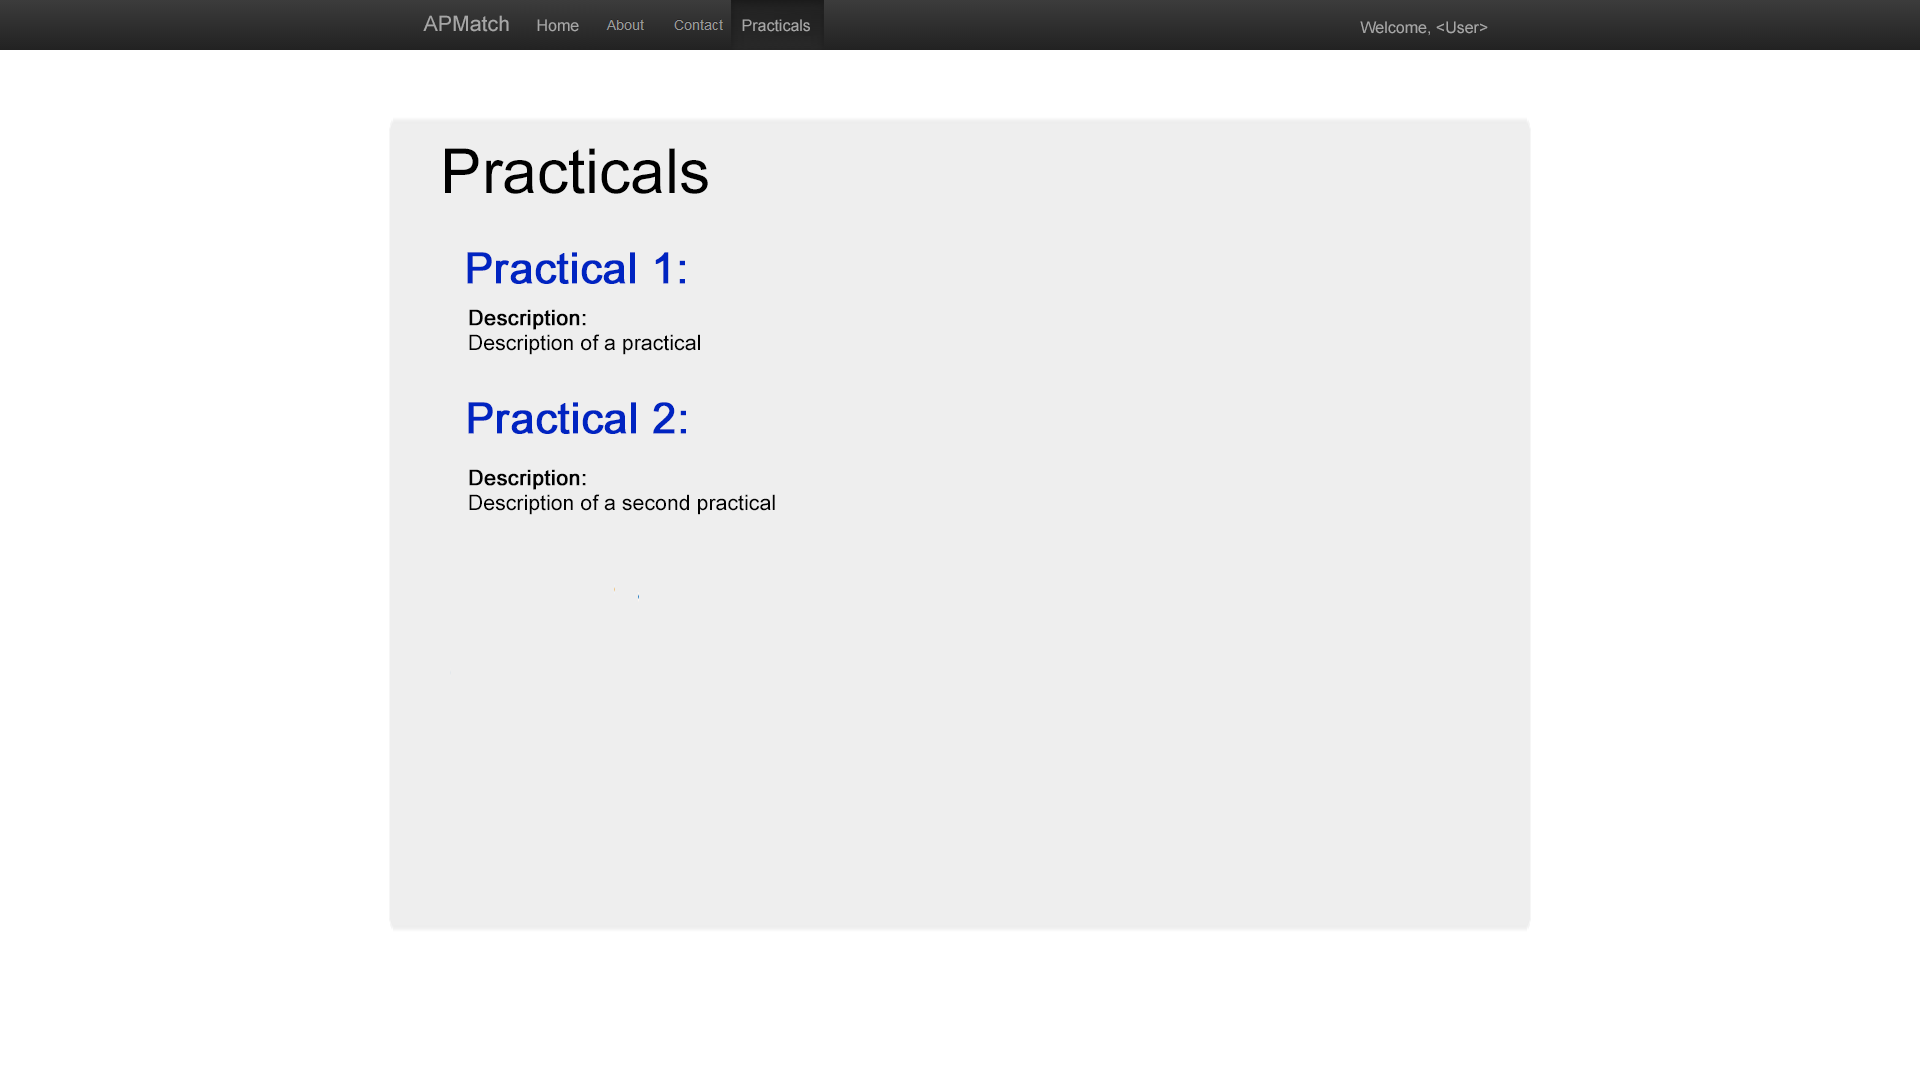
\includegraphics[width=\textwidth, frame]{images/mockup_practical_overview}
    \caption{Interface for the practical overview page}
    \label{mockup_practical_overview}
\end{figure}

\begin{figure}[H]
    \centering
    \captionsetup{justification=centering}
    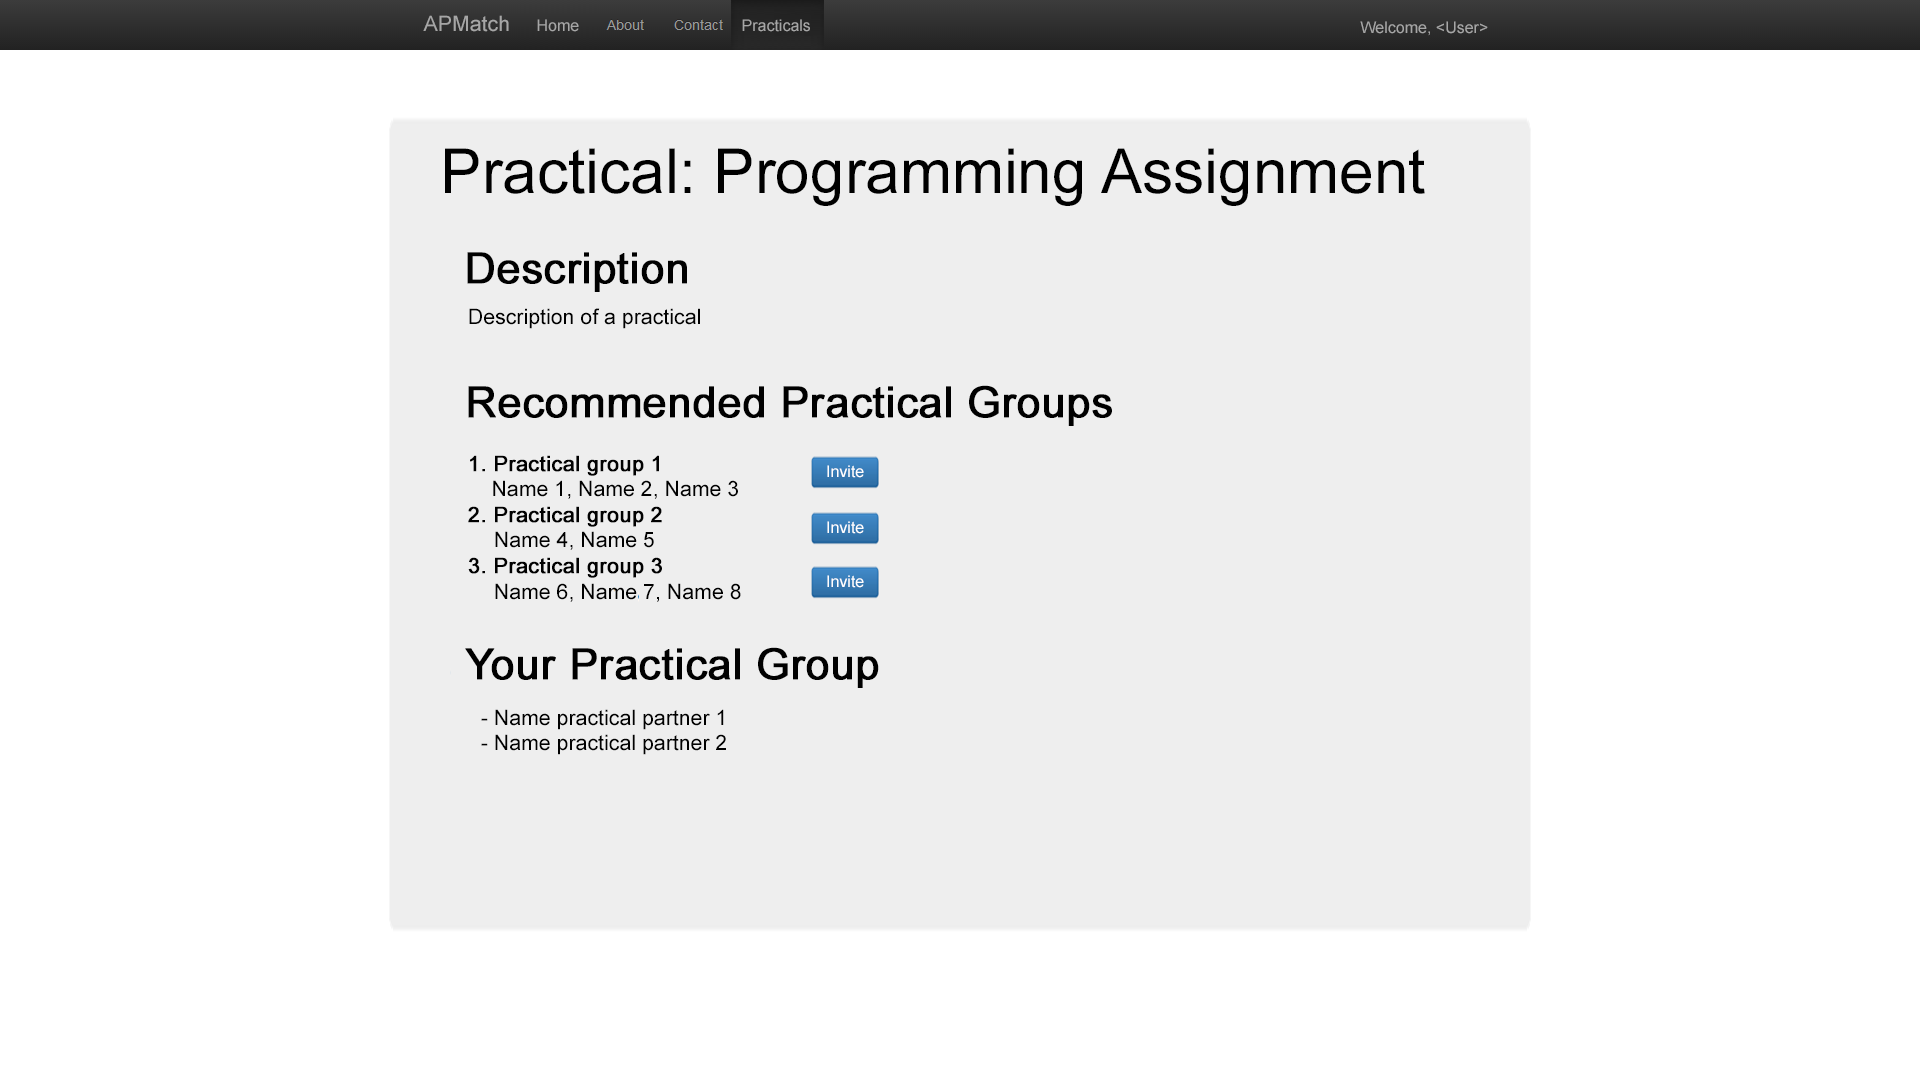
\includegraphics[width=\textwidth, frame]{images/mockup_practical}
    \caption{Interface for the practical page}
    \label{mockup_practical}
\end{figure}
